\documentclass[UTF8,a4paper]{article}
\usepackage{fancyhdr}
\usepackage{ctex}
\usepackage{amsmath}
\usepackage{listings}
\usepackage{color}
\usepackage{graphics}
\usepackage{graphicx}
\lstset{ %
	extendedchars=false,            % Shutdown no-ASCII compatible
	language=Matlab,                % choose the language of the code
	basicstyle=\small\sf,    % the size of the fonts that are used for the code
	tabsize=3,                            % sets default tabsize to 3 spaces
	numbers=left,                   % where to put the line-numbers
	numberstyle=\tiny,              % the size of the fonts that are used for the line-numbers
	stepnumber=1,                   % the step between two line-numbers. If it's 1 each line
	% will be numbered
	numbersep=5pt,                  % how far the line-numbers are from the code   %
	keywordstyle=\color[RGB]{33,33,234},               % keywords
	commentstyle=\color[RGB]{0,0,0},    % comments
	stringstyle=\color[rgb]{0.170,0.187,0.102},      % strings
	backgroundcolor=\color{white}, % choose the background color. You must add \usepackage{color}
	showspaces=false,               % show spaces adding particular underscores
	showstringspaces=false,         % underline spaces within strings
	showtabs=false,                 % show tabs within strings adding particular underscores                frame = single,         % adds a frame around the code
	captionpos=b,                   % sets the caption-position to bottom
	breaklines=true,                % sets automatic line breaking
	breakatwhitespace=false,        % sets if automatic breaks should only happen at whitespace
	title=\lstname,                 % show the filename of files included with \lstinputlisting;
	% also try caption instead of title
	mathescape=true,escapechar=?    % escape to latex with ?..?
	escapeinside={\%*}{*)},         % if you want to add a comment within your code
	%columns=fixed,                  % nice spacing
	%morestring=[m]',                % strings
	%morekeywords={%,...},%          % if you want to add more keywords to the set
	%    break,case,catch,continue,elseif,else,end,for,function,global,%
	%    if,otherwise,persistent,return,switch,try,while,...},%
}
\pagestyle{fancy}
\lhead{}
\chead{}
\rhead{\bfseries The Matlab Homework week 8}
\lfoot{}
\cfoot{\thepage}
\rfoot{}
\renewcommand{\headrulewidth}{0.4pt}
\begin{document}
\begin{center}
    \textbf{\LARGE{Matlab Homework week 8}}\\[0.5cm]
    \normalsize{庄震丰 22920182204393}\\[0.5cm]
    \large{Nov. $21^{st}$, 2019}
\end{center}
\section{Convolution}
\subsection{Description}
Calulate the Convolution of two signals in two methods as follow:
\begin{center}
    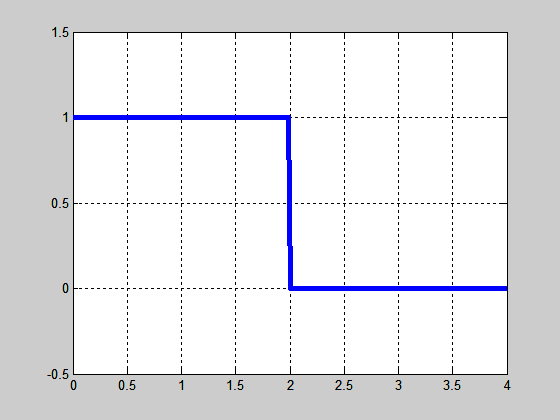
\includegraphics[scale=0.4]{T-1.png}
    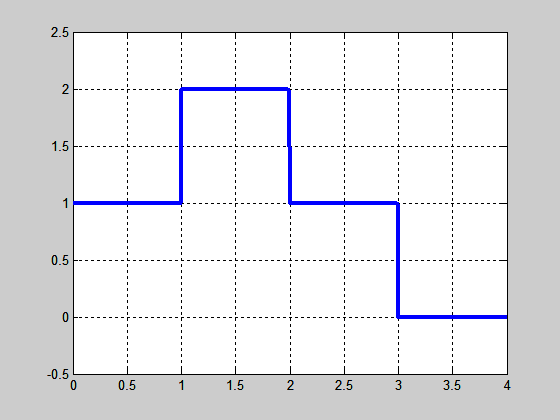
\includegraphics[scale=0.4]{T-1-2.png}\\	
	\textit{Signals $f_1,f_2$}
\end{center}
\subsection{Codes and result}
\textbf{symbolic method}
\begin{lstlisting}
    syms t tao;
    y1=heaviside(-t+2);
    y2=heaviside(t-1)-heaviside(t-2)+heaviside(-t+3);
    f=subs(y1,t,tao)*subs(y2,t,t-tao);
    ft=int(f,tao,0,t);
    fplot(ft);
    hold on;
    grid on;
    axis([-4,7,-1,5])
    title('$f_1*f_2$','Interpreter','Latex')
    xlabel('t');
    ylabel('f');
    legend('signal')
\end{lstlisting}
\textbf{numberical method}
\begin{lstlisting}

    clear all
    dt=0.01;
    t1=0:dt:5;
    t2=0:dt:5;
    f1=heaviside(-t1+2);
    f2=heaviside(t2-1)-heaviside(t2-2)+heaviside(-t2+3);
    f=conv(f1,f2)*dt;
    t0=t1(1)+t2(2);
    t3=length(t1)+length(t2)-2;
    t=t0:dt:t3*dt+t0;
    plot(t,f);
    hold on;
    grid on;
    axis([-4,7,-1,5])
    title('$f_1*f_2$','Interpreter','Latex')
    xlabel('t');
    ylabel('f');
    legend('signal')
\end{lstlisting}
\textbf{result}\\
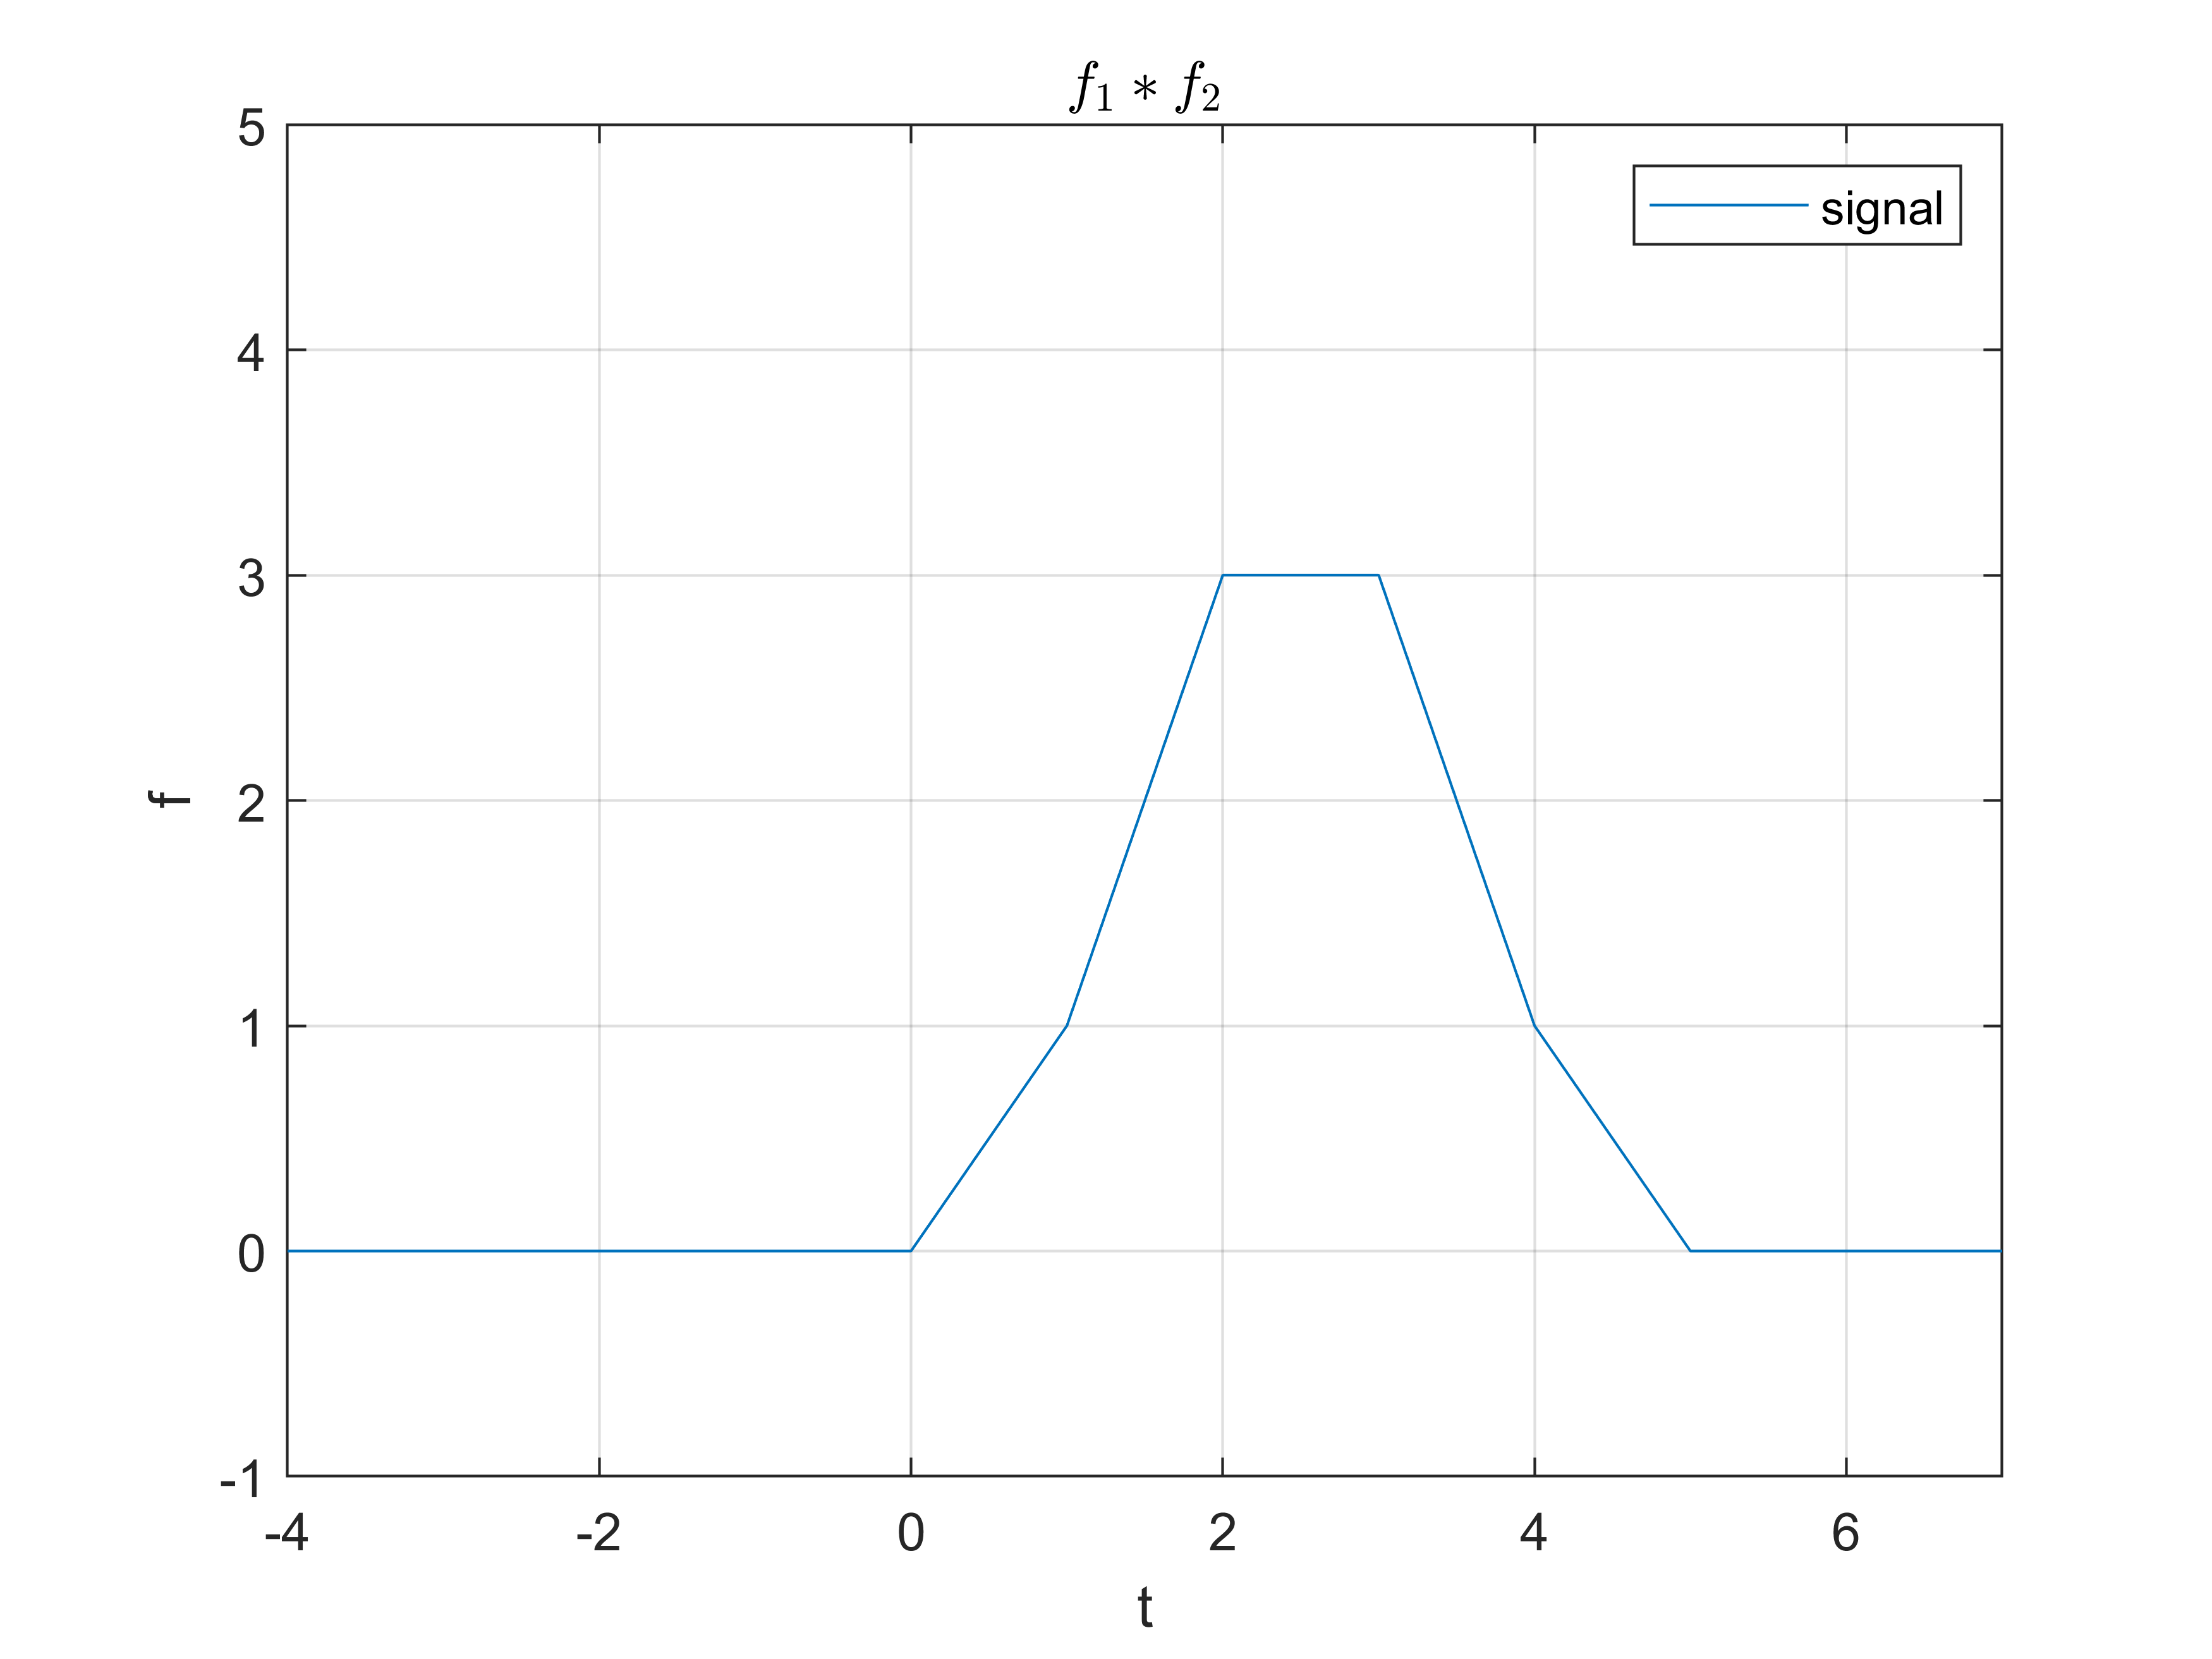
\includegraphics[scale=0.8]{T1.png}
\newpage
\section{Convolution two}
\subsection{Description}
Calulate the Convolution of four signals in two methods as follow:
\begin{center}
    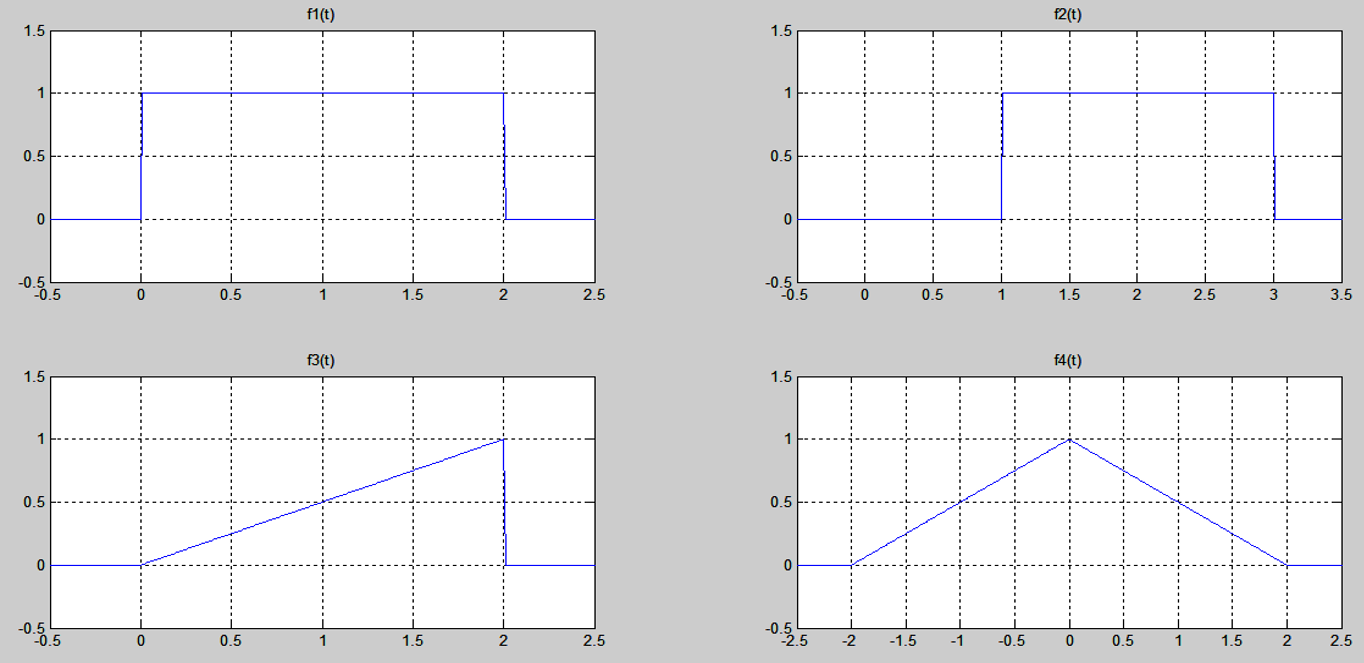
\includegraphics[scale=0.6]{T-2.png}
	\textit{Signals $f_1-f_4$}
\end{center}
$$
\begin{aligned}
f_1(t)*f_2(t),f_1(t)*f_3(t),f_1(t)*f_4(t)\\
f_2(t)*f_3(t),f_2(t)*f_4(t),f_3(t)*f_4(t)\\
\end{aligned}
$$
\subsection{Codes and result}
\textbf{symbolic method}
\begin{lstlisting}
    
syms t tao;
y1=heaviside(t)-heaviside(t-2);
y2=heaviside(t-1)-heaviside(t-3);
y3=1/2*t*(heaviside(t)-heaviside(t-2));
y4=(1/2*t+1)*(heaviside(t+2)-heaviside(t))+(-1/2*t+1)*(heaviside(t)-heaviside(t-2));
figure(2)
subplot(2,2,1)
fplot(y1);
subplot(2,2,2)
fplot(y2);
subplot(2,2,3)
fplot(y3);
subplot(2,2,4)
fplot(y4);
figure(1)
f=subs(y1,t,tao)*subs(y2,t,t-tao);
ft=int(f,tao,-inf,t);
subplot(3,2,1)
fplot(ft);
axis([-8,8,-1,5]);
grid on;
title('$f_1(t)*f_2(t)$','Interpreter','Latex');
subplot(3,2,2);
f=subs(y1,t,tao)*subs(y3,t,t-tao);
ft=int(f,tao,-inf,t);
fplot(ft);
grid on;
title('$f_1(t)*f_3(t)$','Interpreter','Latex');
subplot(3,2,3);
grid on;
f=subs(y1,t,tao)*subs(y4,t,t-tao);
ft=int(f,tao,-inf,t);
fplot(ft);
title('$f_1(t)*f_4(t)$','Interpreter','Latex');
subplot(3,2,4);
f=subs(y2,t,tao)*subs(y3,t,t-tao);
ft=int(f,tao,-inf,t);
fplot(ft);
grid on;
title('$f_2(t)*f_3(t)$','Interpreter','Latex');
subplot(3,2,5);
f=subs(y2,t,tao)*subs(y4,t,t-tao);
ft=int(f,tao,-4,t);
fplot(ft);
title('$f_2(t)*f_4(t)$','Interpreter','Latex');
grid on;
subplot(3,2,6);
f=subs(y3,t,tao)*subs(y4,t,t-tao);
ft=int(f,tao,-inf,t);
fplot(ft);
grid on;
title('$f_3(t)*f_4(t)$','Interpreter','Latex');
\end{lstlisting}
\textbf{numberical method}
\begin{lstlisting}
    clear all;
    dt=0.01;
    t=0:dt:3;
    f1=heaviside(t)-heaviside(t-2);
    f2=heaviside(t-1)-heaviside(t-3);
    f3=1/2*t.*(heaviside(t)-heaviside(t-2));
    f4=(1/2*t+1).*(heaviside(t+2)-heaviside(t))+(-1/2*t+1).*(heaviside(t)-heaviside(t-2));
    subplot(3,2,1)
    f=conv(f1,f2)*dt;
    t=0:dt:6;
    plot(t,f);
    grid on;
    title('$f_1(t)*f_2(t)$','Interpreter','Latex');
    subplot(3,2,2)
    f=conv(f1,f3)*dt;
    t=0:dt:6;
    plot(t,f);
    grid on;
    title('$f_1(t)*f_3(t)$','Interpreter','Latex');
    subplot(3,2,3)
    f=conv(f1,f4)*dt;
    t=0:dt:6;
    plot(t,f);
    grid on;
    title('$f_1(t)*f_4(t)$','Interpreter','Latex');
    subplot(3,2,4);
    f=conv(f2,f3)*dt;
    t=0:dt:6;
    plot(t,f);
    grid on;
    title('$f_2(t)*f_3(t)$','Interpreter','Latex');
    subplot(3,2,5)
    f=conv(f2,f4)*dt;
    t=0:dt:6;
    plot(t,f);grid on;
    title('$f_2(t)*f_4(t)$','Interpreter','Latex');
    subplot(3,2,6)
    f=conv(f1,f2)*dt;
    t=0:dt:6;
    plot(t,f);
    title('$f_3(t)*f_4(t)$','Interpreter','Latex');
\end{lstlisting}
\textbf{result}\\
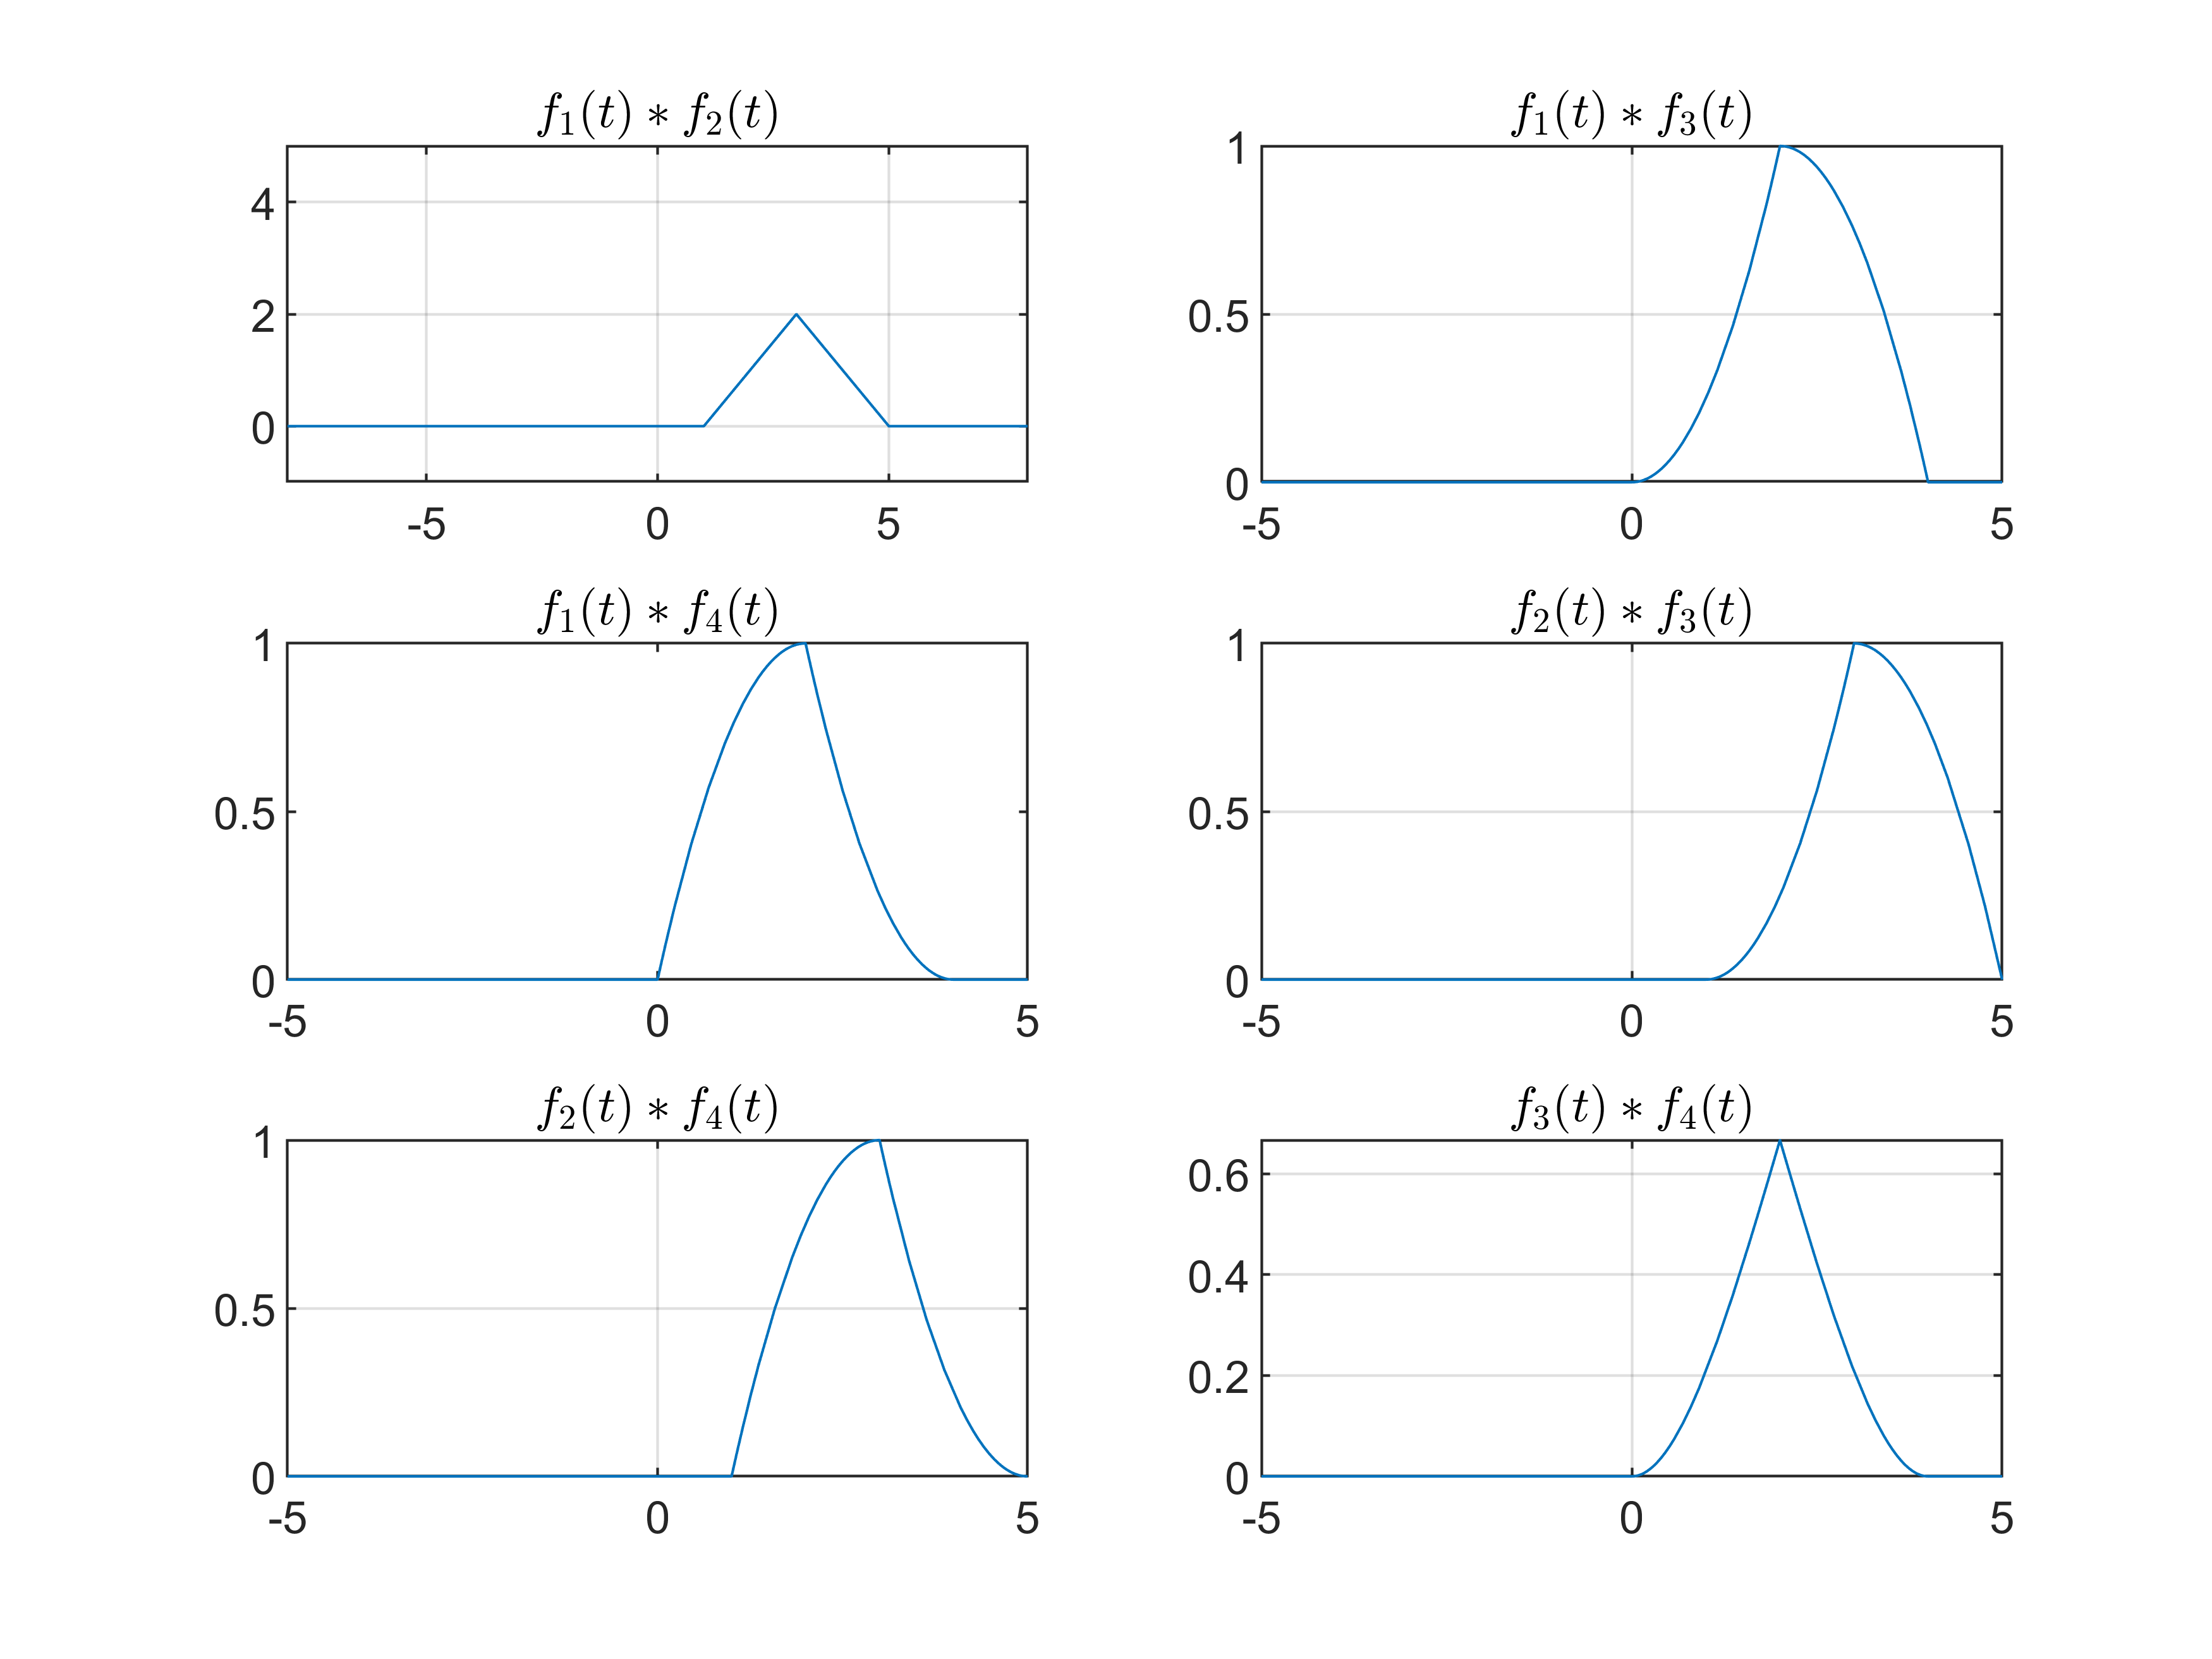
\includegraphics[scale=0.8]{T2.png}
\section{Convolution Three}
\subsection{Description}
Calulate the Convolution of two signals in two methods as follow:
$$
\begin{aligned}
    f_1(t)=u(t)-u(t-2)\\
    f_2(t)=e^{-3t} ~(0<t<7)
\end{aligned}
$$
\subsection{Codes and result}
\textbf{symbolic method}
\begin{lstlisting}
    clear all;
    syms t tao;
    f1=heaviside(t)-heaviside(t-2);
    f2=exp(-3*t)*(heaviside(t)-heaviside(t-7));
    f=int(subs(f1,t,tao)*subs(f2,t,t-tao),tao,-inf,t);
    fplot(f)
\end{lstlisting}
\textbf{numberical method}
\begin{lstlisting}
    clear all;
    dt=0.01;
    t=0:dt:7;
    f1=heaviside(t)-heaviside(t-2);
    f2=exp(-3*t).*(heaviside(t)-heaviside(t-7));
    f=dt*conv(f1,f2);
    t=0:dt:14;
    plot(t,f)\end{lstlisting}
\textbf{result}\\
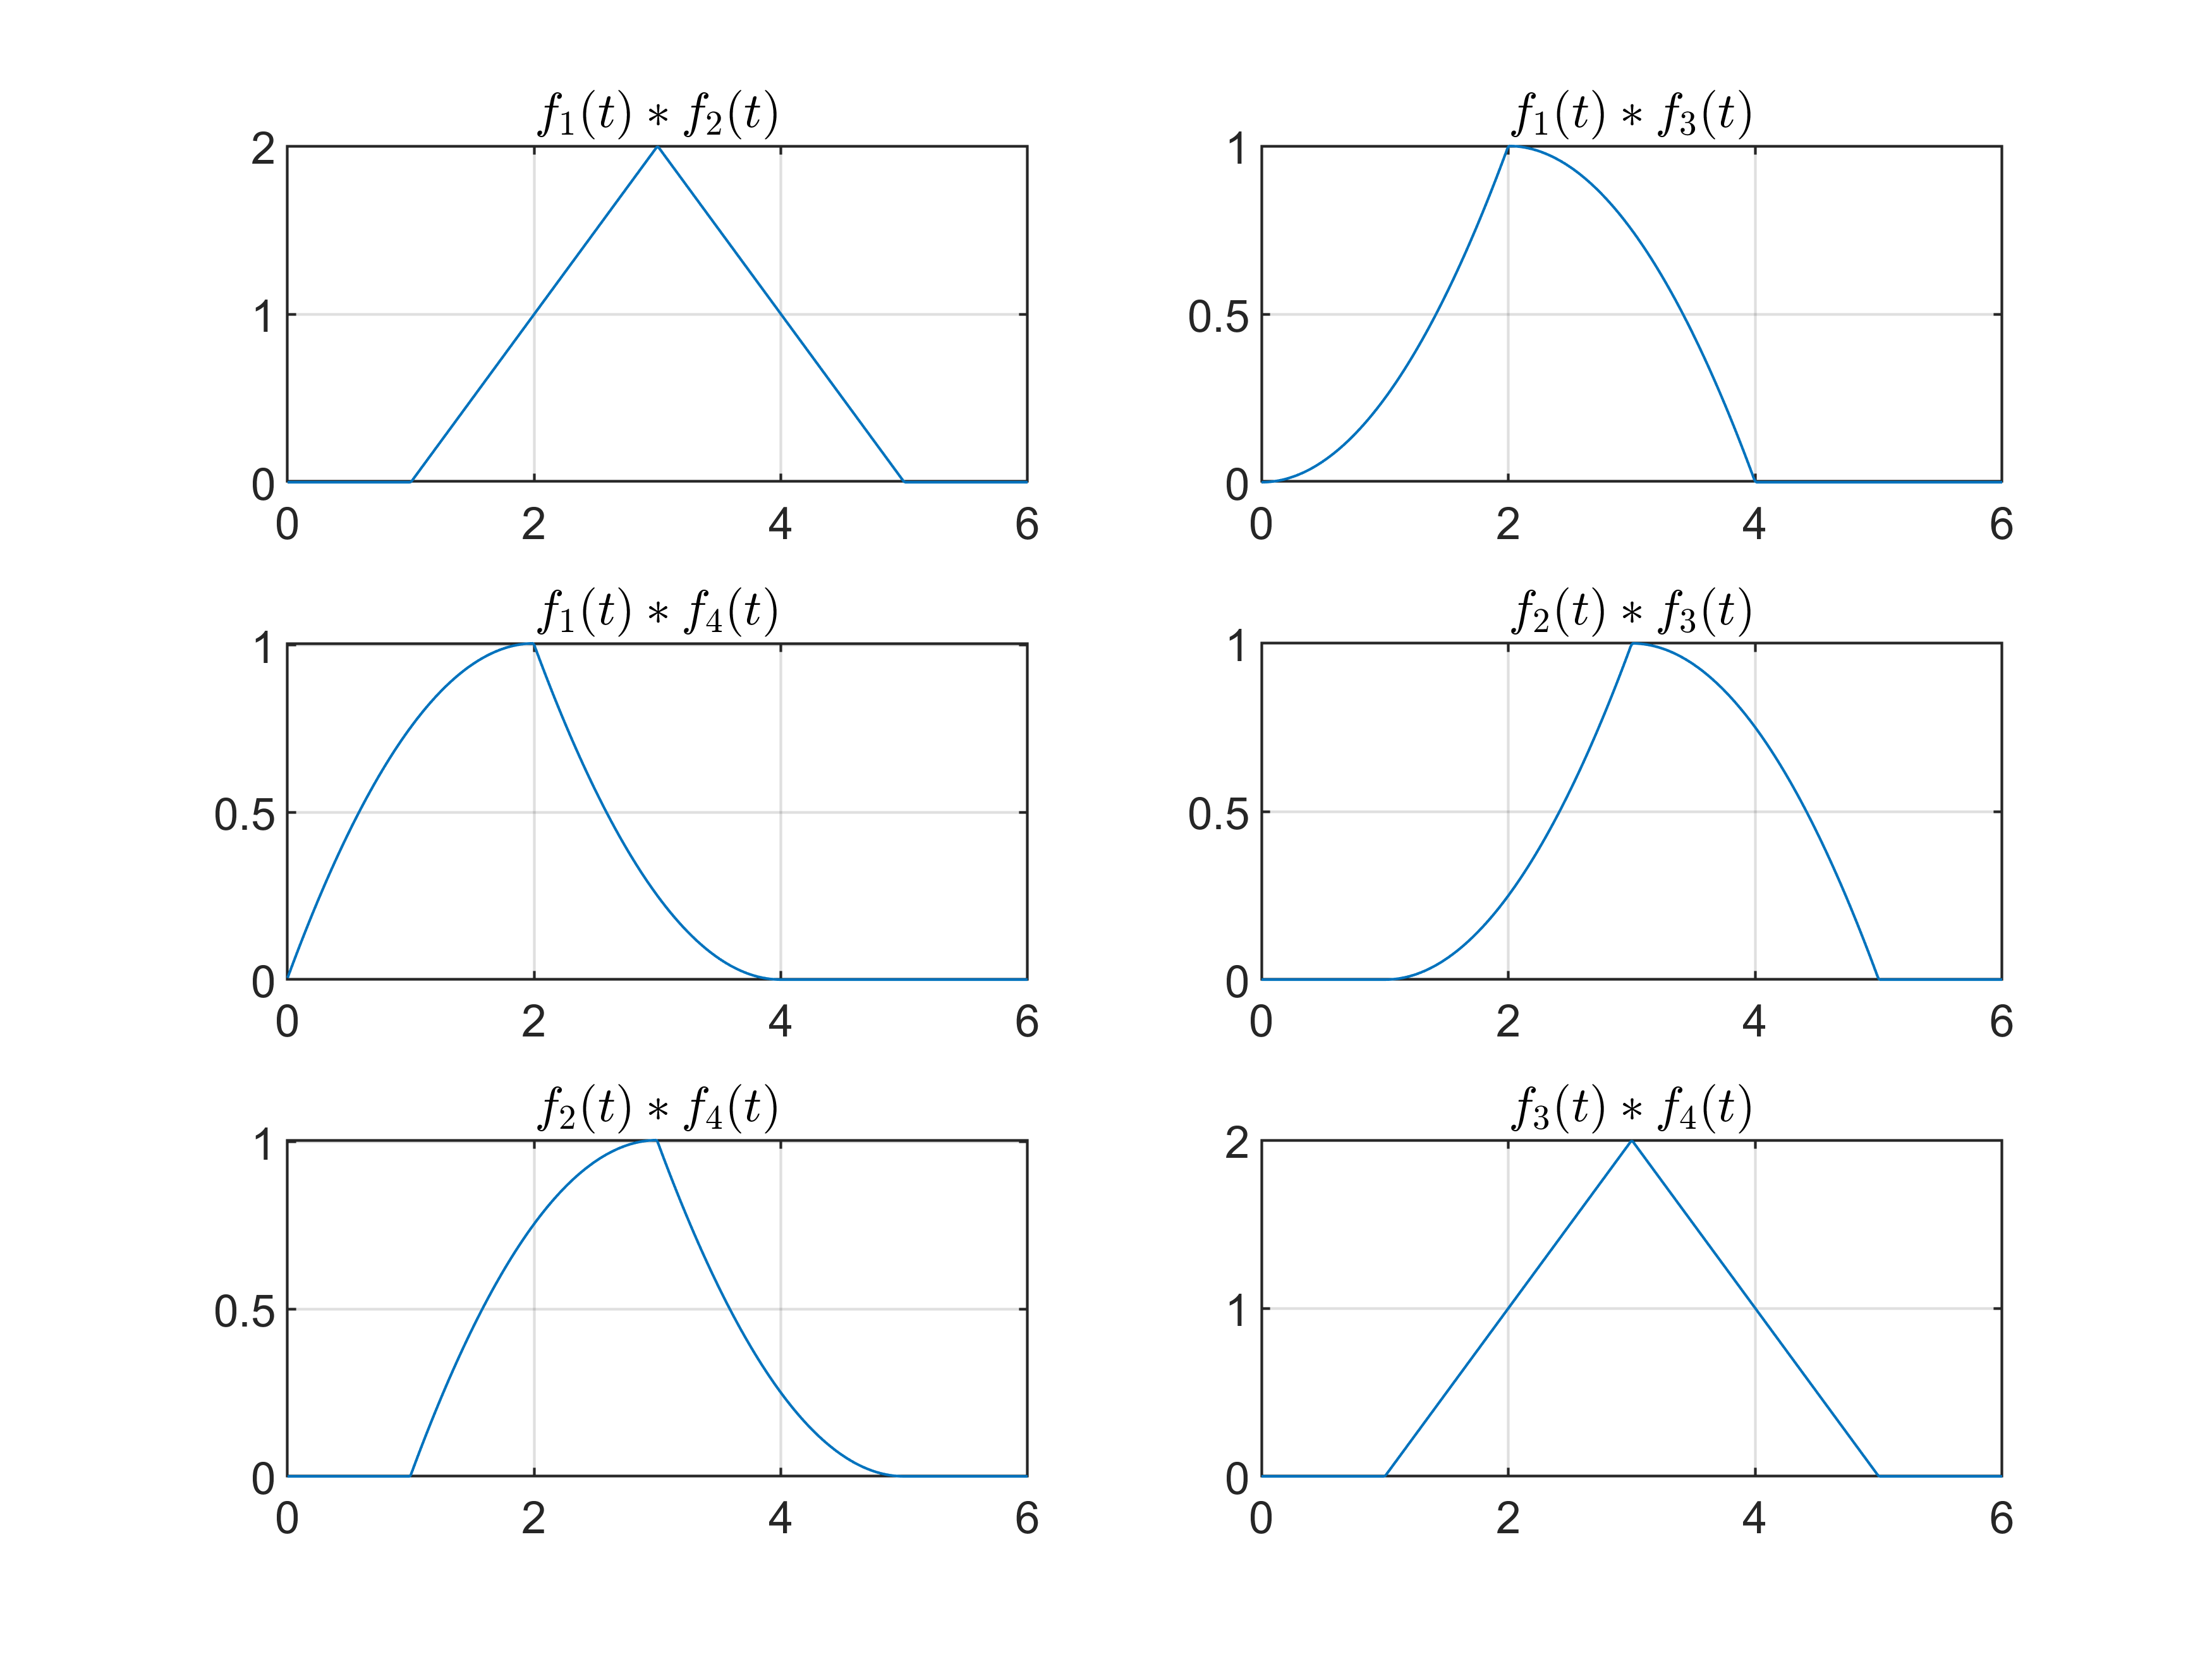
\includegraphics[scale=0.8]{T3.png}
\end{document}